\documentclass[10pt,a4paper]{article}
\usepackage[utf8]{inputenc}
\usepackage{amsmath}
\usepackage{amsfonts}
\usepackage{amssymb}
\usepackage{graphicx}
%\usepackage[colorlinks=true]{hyperref}
\usepackage{hyperref}
\author{Leandro M. Arancibia$^{\dagger\ddagger}$  \and  Andrés I. Bertoni$^{\dagger\ddagger}$ \and Cristián G. Sánchez$^{\dagger}$ \and Alejandro M. Lobos$^{\dagger\,*}$  \\ 
\\ $^\dagger$Instituto Interdisciplinario de Ciencias Básicas (ICB-CONICET),\\ Universidad Nacional de Cuyo,\\ Padre Jorge Contreras 1300, Mendoza 5502, Argentina \\\\
$^\ddagger$ \begin{normalsize}
These authors contributed equally to this work and are listed in alphabetical order.
\end{normalsize}\\
(\begin{normalsize}
$^*$ Corresponding author.~E-mail:~ \texttt{alejandro.martin.lobos@gmail.com}
\end{normalsize})
}
\title{Towards electrical domain-wall control in polyacetylene-based electronic nanodevices}
\begin{document}
\maketitle
\begin{abstract}
We theoretically propose a polymer-based nano-device consisting of a single \textit{trans}-polyacetylene (tPA) molecule capacitively coupled to external voltage gates. We model the integrated device using a Su-Schrieffer-Heeger (SSH)-like Hamiltonian, and we demonstrate the emergence of localized domain walls (DWs) with quantized charges (i.e., soliton excitations) localized at the gates. Interestingly, by increasing the applied voltage, multiple discrete charges can be accumulated, which may be useful for potential technological applications. Exploiting the topological character of the solitonic excitations of tPA, this device can be considered as an organic-based quantum dot with a very large and robust quantized charge.
\end{abstract}

\section{Introduction}
\label{sec:intro}
% TODO: write your article here. 
The emergent area of synthetic organic metals based on polymers is an important field at the intersection of chemistry and physics, with interest
both from the perspective of fundamental research as well as for organic electronics and other technological applications ~\cite{Farchioni_Grosso_Organic_electronic_metals_book}. Historically, \textit{trans}-polyacetylene (tPA), a linear chain of carbon atoms with alternating single and double bonds, was identified as the first organic conductor\cite{Heeger88_Solitons_in_conducting_polymers, Su79_Solitons_in_polyacetylene}. 

A key aspect of tPA is its double-degenerate ground state corresponding to the two possible ways to accommodate the (Peierls) dimerization pattern of single and double bonds. In its ground state, the system is an insulator characterized by a (Peierls) gap in the single-particle spectrum of excitations. However, tPA can be excited to a soliton-like state
%with mobile charges, thus acting as a conductor, and also potentially localize spin excitations~[REF?]. These conducting excited states 
which features an excess charge bound to lattice deformations known as domain walls (DWs), which bridge two different dimerization patterns, and intra-gap single-electron states linked to the solitonic nature of the excitation. The first experimental evidence of  soliton excitations in tPA was indirectly established via optical spectroscopy\cite{sethna1982photoinduced, blanchet1983photoexcitations} and magnetic electron paramagnetic resonance (EPR) experiments\cite{goldberg1979electron, weinberger1980electron}.

Recent progress in nano-fabrication methods has shown the possibility to synthesize linear chains of tPA on clean metallic surfaces\cite{Wang19_Solitons_in_individual_PA_molecules}. In particular, in Ref.\cite{Wang19_Solitons_in_individual_PA_molecules} it was possible for the first time to address and study a single tPA molecule deposited on a Cu(110) surface, via scanning tunneling microscopy (STM) techniques. Experimental signatures in the STM differential conductance $dI/dV$ indicate the presence of a trapped electronic state at the DW, constituting the first experimental evidence of a charged soliton. Furthermore, the ability to control and manipulate DWs in bi- and tri-layer graphene has been experimentally demonstrated in recent works\cite{Jiang18_Manipulation_of_DWs_in_bi_and_trilayer_graphene}. This type of synthesis stimulated recent proposals of single-molecule nano-devices that use soliton excitations as the main mechanism for electronic transport\cite{HernangomezPerez20_Solitonics_with_PA, park2022creation}.

Motivated by these recent advances, in this work we theoretically demonstrate the possibility to capacitively induce charged DWs (CDWs) in a single tPA molecule, and therefore to control its electronic intra-gap spectrum, allowing interesting functionalities for this class of devices. The proposed nano-device, depicted schematically in Fig. \ref{fig:device}, consists of a linear tPA molecule deposited on an insulating film (e.g., $\text{SiO}_2$) under which gate voltages are applied. These gate voltages are assumed to locally modify the chemical potential of the exposed molecular segments via capacitive coupling and induce the nucleation of CDWs, which can be regarded as a local doping of the molecule at the gate region. In other words, we propose that the strong electron-phonon coupling present in organic $\pi$-conjugated molecules can be exploited to generate charge carriers or spin excitations at any desired region within the polymer. Although this device effectively behaves as a molecular quantum dot (QD) that hosts quantized charges, we show that it is markedly more localized and superior in robustness to disorder and other local perturbations over a wide range of parameters due to the topological origin of the DWs.
\begin{figure}
    \centering
    \begin{minipage}[t]{0.35\textwidth}
        \raggedright
        \textbf{(a) } \vspace{1.5cm} \\
        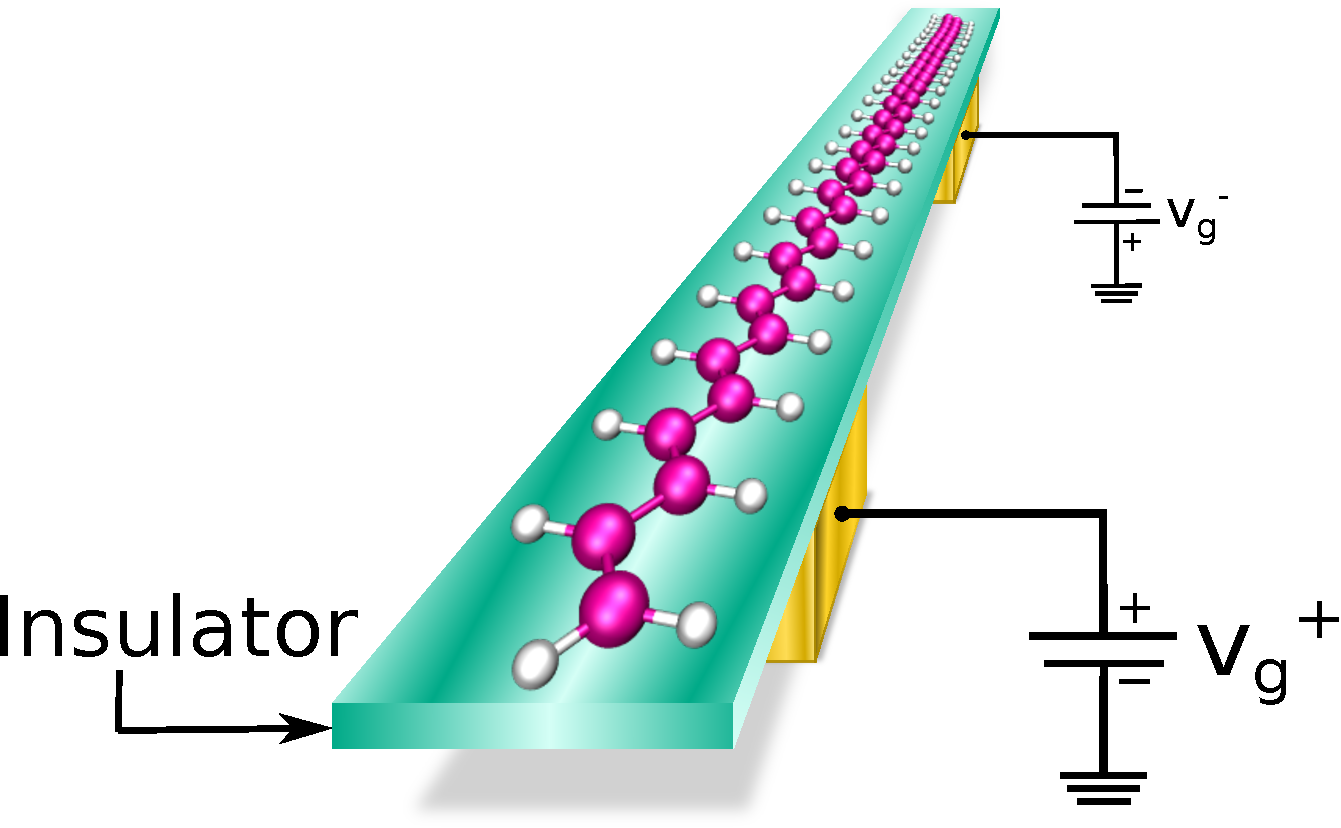
\includegraphics[width=\textwidth]{figures/device.pdf}
    \end{minipage}
    \hfill
    \begin{minipage}[t]{0.6\textwidth}
        \raggedright
        \textbf{(b)} \\
        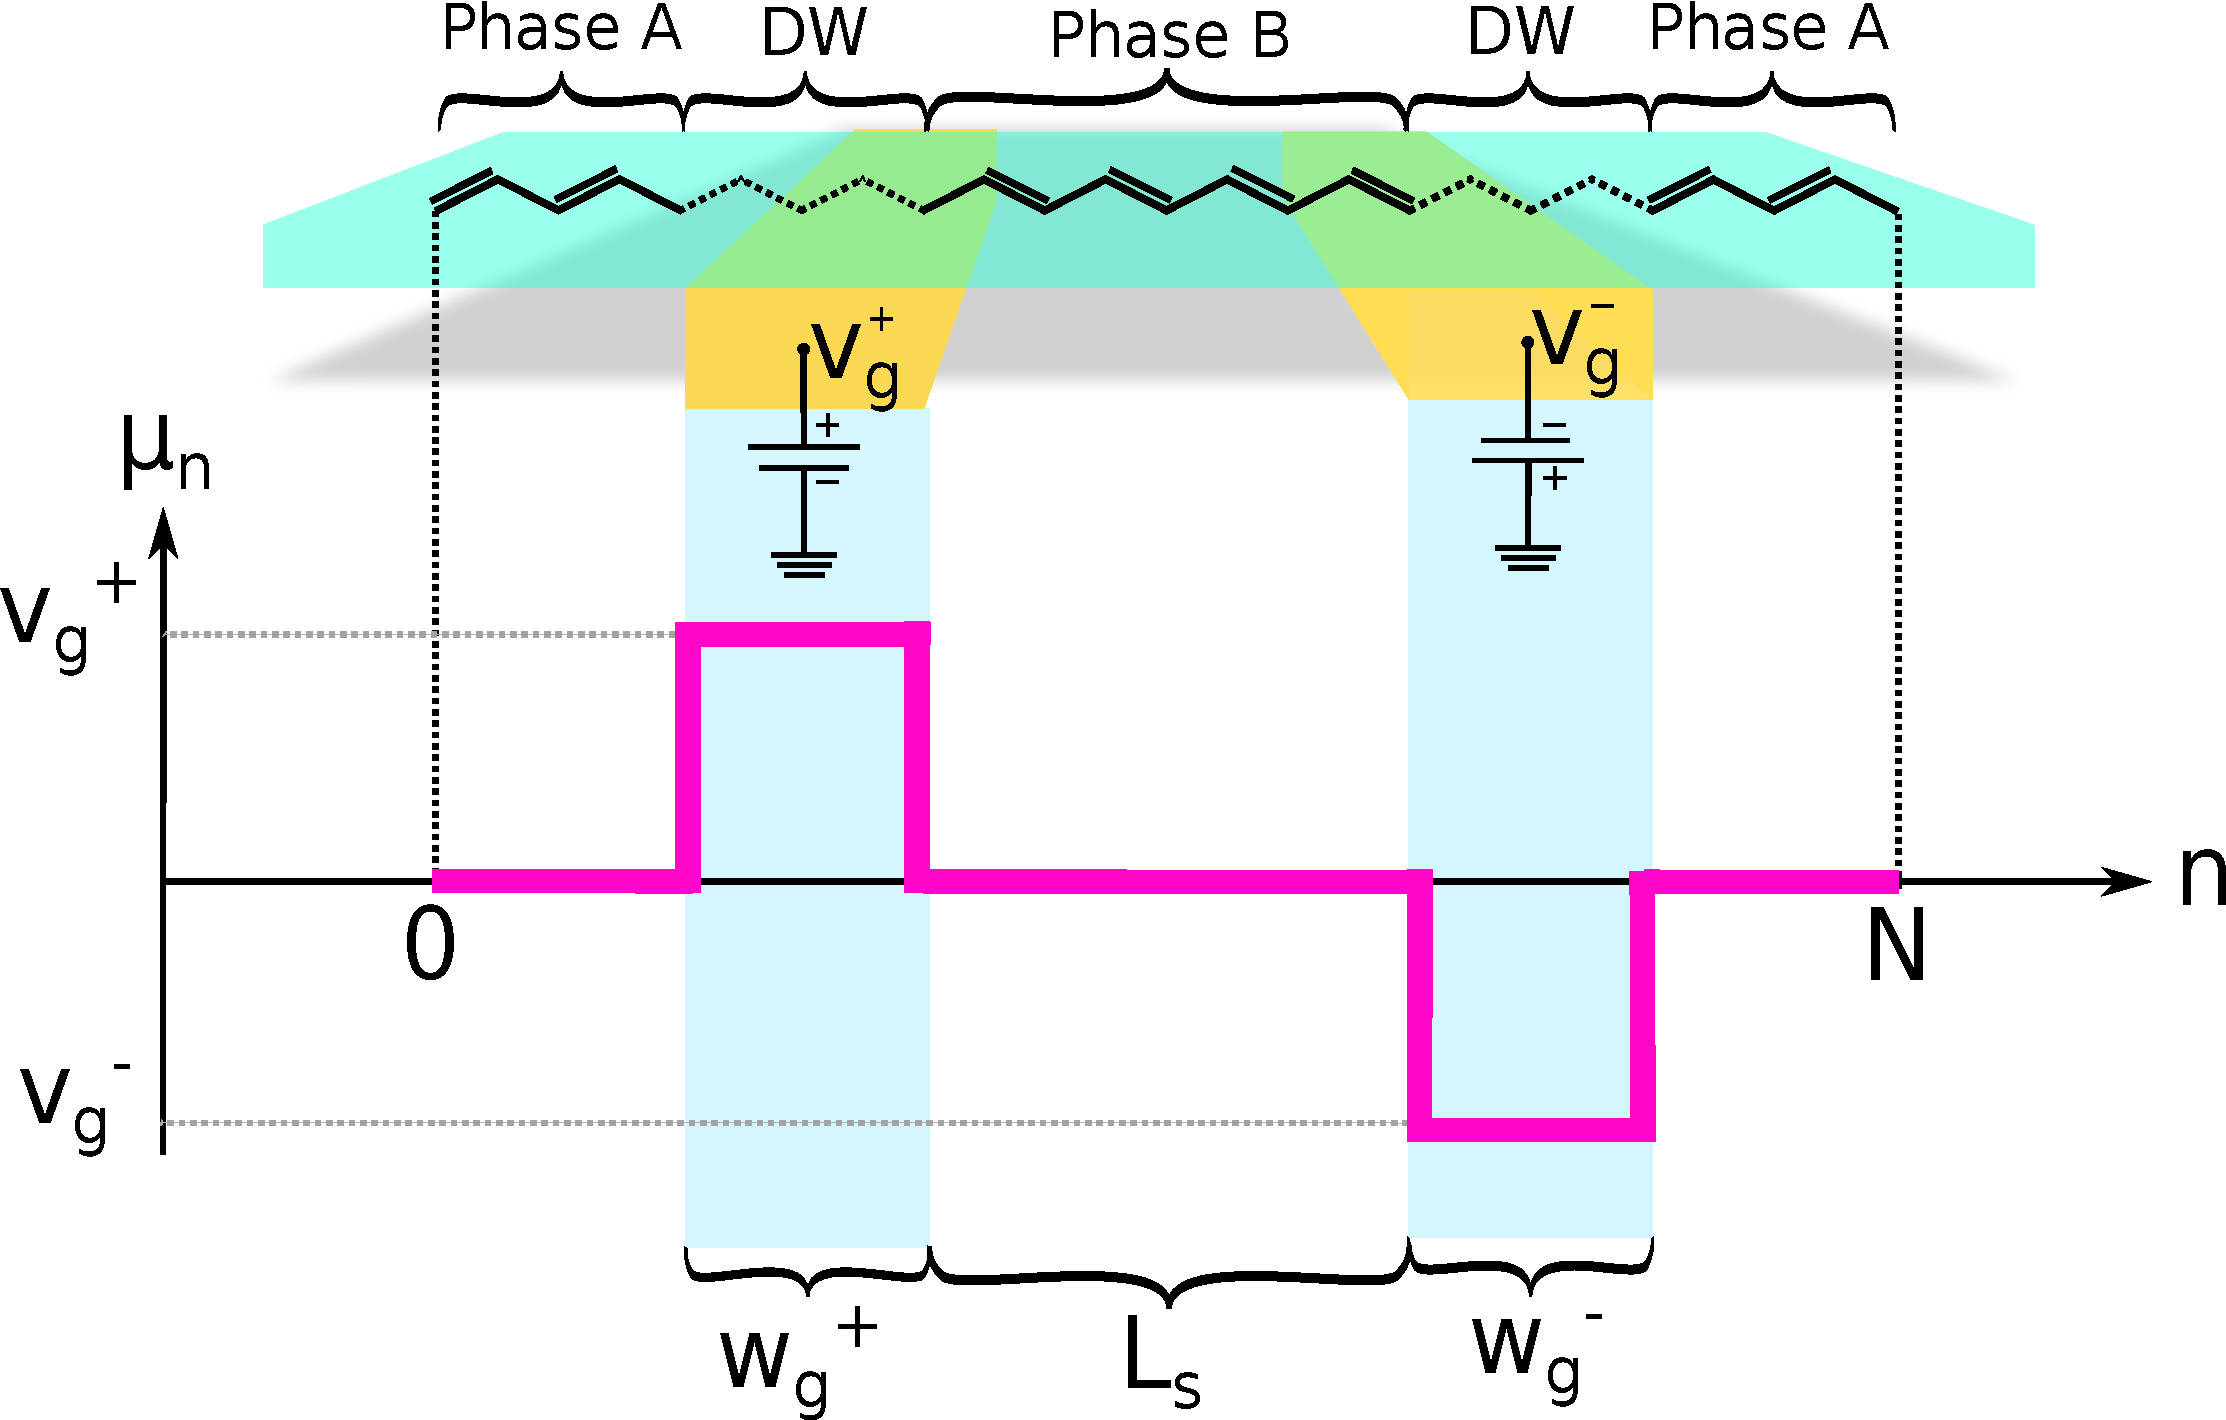
\includegraphics[width=\textwidth]{figures/diagram.pdf}
    \end{minipage}
    \caption{Schematics of the proposed tPA-based nano-device: a single finite trans-polyacetylene (tPA) molecule is deposited on an insulating thin film (e.g. $\text{SiO}_2$). The system is capacitively coupled to two independently adjustable voltage gates of equal width $w_{g}$ and separated by a distance $L_{s}$, that are connected to opposite voltages $V_{g}^{+}$ and $V_{g}^{-}$ (encoded in a phenomenological site-dependent chemical potential~$\mu_{n}$).}\label{fig:device}
\end{figure}
\section{Model}\label{sec:model}

Illustrated in Fig.~\ref{fig:device}, our model considers a finite, linear tPA chain deposited on an insulating thin film, e.g. silica, with two voltage gates placed underneath so that they are only capacitively coupled to separate regions of the molecule. These gates are connected to external independent voltages that are able to locally control the electron density of the molecular segments by modifying their electro-chemical potential. We model this device by the means of the Su-Schrieffer-Heeger (SSH) Hamiltonian\cite{Heeger88_Solitons_in_conducting_polymers, Su79_Solitons_in_polyacetylene}, with slight modifications to treat open-ended molecular chains\cite{Vos96_SSH_model_finite_length} and to describe the effect of the voltage gates on the electron density. The SSH Hamiltonian is a celebrated model introduced to describe the interaction of $\pi$-conjugated electrons with the classical ionic degrees of freedom in linear polyalkenes. This rather simple model successfully accounts for many of the experimentally observed properties of tPA, such as the existence of a Peierls dimerization gap, and theoretically explains the emergence of fractional solitons \cite{Farchioni_Grosso_Organic_electronic_metals_book, Heeger88_Solitons_in_conducting_polymers}. The SSH model is one of the most paradigmatic models in condensed-matter physics, since it realizes the simplest example of a topological insulator in one dimension\cite{Bernevig_book_TI_TSC, Asboth16_Short_course_on_TIs}. 

Explicitly, we have
%
\begin{align}
\hat{H} = \hat{H}_{\textbf{el}} + \hat{H}_{\textbf{latt}} \, ,
\end{align}
%
where the electronic Hamiltonian, $\hat{H}_{\textbf{el}}$, describes both the electron-lattice and the electron-gate interaction, and the classical Hamiltonian, $\hat{H}_{\textbf{latt}}$, describes the elastic interaction between the (CH) groups:
%
\begin{align}
\hat{H}_{\textbf{el}} = & \sum_{n=1,s}^{N_{s}-1} \left[ -t_{0} + \alpha \left( u_{n+1} - u_{n} \right) \right] c_{n,s}^{\dagger} \, c_{n+1,s} + \textbf{H.c.} + \sum_{n=1,s}^{N_{s}} \mu_n \, c_{n,s}^{\dagger} \, c_{n,s} \, , \label{eq:H_el} \\
\hat{H}_{\textbf{latt}} = & \sum_{n=1}^{N_{s}} \frac{p_{n}^{2}}{2M} + \sum_{n=1}^{N_{s}-1} \frac{K}{2} \left( u_{n+1} - u_{n} \right)^{2} - \sum_{n=1}^{N_{s}-1} \Gamma \, (u_{n+1} - u_{n}) \, . \label{eq:H_latt}
\end{align}
%
The first term of Eq.~(\ref{eq:H_el}) describes the electrons in the $\pi$ bands, arising from the $2p_{z}$ orbitals of a tPA molecule with $N_{s}$ (CH) moieties, each one considered a discrete ``site’’ in the chain. The operator $c_{n,s}$ ($c^{\dagger}_{n,s}$) annihilates (creates) an electron with spin $s$ at site $n$. The parameter ${t_{0} = 2.5 \, \textbf{eV}}$ is the hopping integral, ${\alpha = 4.1 \, \textbf{eV}/\textbf{\AA}}$ is the electron-lattice coupling parameter, and $u_{n}$ are the classical variables describing the deviation from equilibrium of the $n$-th site along the chain axis. Essentially, the term in square brackets in Eq.~(\ref{eq:H_el}) is what results from expanding the full hopping integral up to first order, with a small parameter $(u_{n+1} - u_{n} )$.

The last term of~$\hat{H}_{\textbf{el}}$ introduces the effect of the external gate voltages. In order to simplify the theoretical calculations, we choose to work in the microcanonical ensemble, where the number of electrons $N_{\textbf{el}}$ has been set assuming an overall half-filling condition, i.e. ${N_{\textbf{el}} = N_{s}}$ with $N_{s}$ being the total number of sites in the chain; this condition is ensured by constraining the electronic solutions in all the steps of the variational minimization process. As a result of imposing global half-filling (i.e., charge neutrality under our assumptions), the effect of the gate voltages is limited to the redistribution of electronic charge within the system, favoring an excess of electron density at some sites at the expense of its depletion at other points in the chain. The microcanonical constraint is equivalent to disallowing electron transfer events, or any other direct interaction, through or with the insulating film, which therefore acts as a decoupling layer. While a single-gate version of the device may be  simpler to realize from the  experimental point of view, it becomes theoretically more complicated as it necessarily would involve interaction and equilibration with an external charge reservoir (i.e., grand-canonical ensemble). However, placing the gates sufficiently separated from each other allows to avoid direct interaction between them and enables us to infer the properties of a single-gate device. In addition, in what follows we assume exact anti-symmetric gates (i.e, identical to each other but with opposite voltages). Accordingly, as shown in Fig.~\ref{fig:device}(b), we define two distinct gate regions~$g^{+}$ and~$g^{-}$, each spanning~$w_{g}$ sites, which are associated with constant voltages $+V_{g}$ and $-V_{g}$, respectively, with ${V_{g} > 0}$. In Eq.~(\ref{eq:H_el}), these external gate voltages are encoded in a phenomenological site-dependent chemical potential~$\mu_{n}$, such that ${\mu_{n} = +V_{g},~ n \in g^{+}}$ and ${\mu_{n} = -V_{g},~ n \in g^{-}}$, being zero for non-gate sites (${\mu_{n} = 0 ,~ n \notin \{g^{+}, g^{-}\}}$). The anti-symmetry of the external perturbation is crucial for extrapolating our results to the case of a single gate in open conditions, since it would ensure the occurrence of simultaneous and (anti-)symmetric events involving electrons and lattice.

The first term in Eq.~\ref{eq:H_latt} provides a classical description for the lattice ions, where ${M = 2.152} \, {\times 10^{-26} \, \textbf{Kg}}$ is the mass of each site (i.e., of the $\textbf{(CH)}_{n}$ groups) and ${K = 21 \, \textbf{eV}/\textbf{\AA}^{2}}$ is the effective spring force constant of the C-C bonds. As was already noted by Su \textit{et al.}\cite{Su80_Dynamics_of_solitons_in_PA}, and by Vanderbilt \textit{et al.}\cite{Vanderbilt80_Disorder_in_tPA}, in the open-boundary SSH model there is a tendency for the chain to shrink under the effect of the unconstrained electronic linear coupling to the $\pi-$electrons. This is of course an artifact of the SSH model, rooted at the harmonic approximation, that should be solved by more sophisticated treatments (e.g., proper \textit{ab initio} potentials). In order to compensate for this undesired effect while keeping the simplicity of the theoretical modeling, we followed Refs.~\cite{Su80_Dynamics_of_solitons_in_PA, Vanderbilt80_Disorder_in_tPA, Vos96_SSH_model_finite_length} and introduced an additional term, ${\sum_{n=1}^{N_{s}-1} \Gamma \, (u_{n+1} - u_{n}) = \Gamma \, (u_{N_{s}} - u_{1})}$, which applies an explicit ``stretching’’ force to the ends of the chain to compensate for the spurious contraction. We chose ${\Gamma = 5.15 \, \textbf{eV}/\textbf{\AA}}$ in order to reproduce the same bulk properties seen in experiments (i.e. values of the Peierls distortion, gap size, etc.). Since the stretching term only introduces distortions that are localized at the ends of the chain, it does not affect our conclusions based on sites that are away from the edges of the molecule. 

For this work, we considered a tPA molecule containing two hundred carbon atoms (i.e., ${N_{s} = 200}$) that is capacitively coupled to a pair of anti-symmetric voltage gates of width ${w_{g} = 40 \, a \approx 5 \, \textbf{nm}}$ at distance of ${L_{s} = 80 \, a \approx 10 \, \textbf{nm}}$; these values are within experimental reach using, e.g., electron-beam lithography techniques. Throughout this study, we have adjusted the gate voltages up to ${V_{g} = 1.5 \, \textbf{eV}}$.

Previous experimental works using chemical doping techniques reported evidence of charged intra-gap states associated with solitonic or polaronic excitations appearing at random positions along the tPA chain\cite{Heeger88_Solitons_in_conducting_polymers, Chiang77}. Although the underlying physical mechanism is similar, the crucial difference with our case is that we propose a way to induce the electronic doping in a controlled manner, via the nucleation of DWs facilitated by tunable external voltage gates at specific locations of the chain (see Section~\ref{sec:results}). This effect could be exploited in the design of novel organic quantum electronic devices. Due to the topological origin of the induced intra-gap states, we argue that our phenomenological description, although simplistic, is sufficient to capture the main features of the voltage-controlled doping. We also speculate that more sophisticated (even microscopic) descriptions of this system will not qualitatively change our main conclusions.

\section{Methodology}

In order to solve the static problem we focus on the zero temperature case, and employ the Hellmann-Feynman theorem\cite{feynman39}:
%
\begin{equation}\label{eq:Helmann-Feynman}
\frac{\partial E_{\mathrm{GS}}}{\partial R_{n}} = \left\langle \Psi_{\mathrm{GS}} \left| \frac{\partial \hat{H}}{\partial R_{n}} \right| \Psi_{\mathrm{GS}} \right\rangle = 0 \, ,
\end{equation}
%
where $|\Psi_{\mathrm{GS}}\rangle$ is the electronic ground state wavefunction, $E_{\mathrm{GS}}$ is the total ground state energy (i.e., ${\hat{H} \, |\Psi_{\mathrm{GS}}\rangle = E_{\mathrm{GS}} \, |\Psi_{\mathrm{GS}}\rangle}$), and ${R_{n} = na + u_{n}}$ is the position of the $n-$th site along the chain axis, with lattice parameter ${a = 1.22 \, \textbf{\AA}}$. Eq.~(\ref{eq:Helmann-Feynman}) leads to the following system of coupled equations:
%
\begin{align}
+K \, \left( R_{2} - R_{1} - a \right) - \Gamma + \alpha \sum_{s}\sum_{\nu=1}^{\textbf{occ}} \left[ \psi_{\nu,s}^{*}(2) \, \psi_{\nu,s}(1) + \textbf{H.c.} \right] = & \, 0 \, , \label{eq:HF_L} \\
K \, \left( R_{n{+}1} - 2 R_{n} + R_{n{-}1} \right) - \alpha \sum_{s}\sum_{\nu=1}^{\textbf{occ}} \left[ \left( \psi_{\nu,s}^{*}(n{+}1) - \psi_{\nu,s}^{*}(n{-}1) \right) \, \psi_{\nu,s}(n) + \textbf{H.c.} \right] = & \, 0 \, \nonumber \\  \hfill \forall\, n\, \mathrm{such}\, \mathrm{that}\, 1<n<N_{s} \, , \label{eq:HF_mid} \\
-K \, \left( R_{N_{s}} - R_{N_{s}{-}1} - a \right) + \Gamma - \alpha \sum_{s}\sum_{\nu=1}^{\textbf{occ}} \left[ \psi_{\nu,s}^{*}(N_{s}{-}1) \, \psi_{\nu,s}(N_{s}) + \textbf{H.c.} \right] = & \, 0 \, . \label{eq:HF_R}
\end{align}
%
In the above equations, $\psi_{\nu,s}\left(n\right)$ is the probability amplitude of the $\nu$-th eigenstate at the $n$-th site, i.e. ${|\psi_{\nu,s}\rangle \equiv \sum_{n=1}^{N} \psi_{\nu,s}\left(n\right) c^\dagger_{n,s} |0\rangle}$, which satisfies the single-particle eigenvalue equation:
%
\begin{align}\label{eq:eigenvalue}
\hat{H}_{\textbf{el}} \, |\psi_{\nu,s} \rangle = \epsilon_{\nu} \, |\psi_{\nu,s} \rangle \, ,
\end{align}
%
with $\epsilon_{\nu}$ as the corresponding single-particle energy. Moreover, note that summations run over the doubly occupied (``occ’’) one-electron states (since $N_{\textbf{el}}^{\uparrow} = N_{\textbf{el}}^{\downarrow}$ due to the SU(2) symmetry of the model). Note also that Eq.~(\ref{eq:eigenvalue}) is solved for a given specific configuration of the lattice deformation field $R_{n}$; therefore, the set of Eqs.~(\ref{eq:HF_L})-(\ref{eq:eigenvalue}) form a complete set of coupled non-linear equations that must be solved self-consistently. Finally, note that for our model of non-interacting electrons, the electronic ground state is simply written as ${\left| \Psi_{\mathrm{GS}} \right\rangle = \prod_s \prod_{\nu=1}^{N_{\textbf{el}}} c_{\nu,s}^\dagger |0\rangle }$, with the fermionic operators $c_{\nu,s}$ defined as ${c_{\nu,s} = \sum_{n=1}^{N} \psi_{\nu,s}\left(n\right) \, c^\dagger_{n,s} }$.

We have implemented a numerical routine for the energy minimization that starts with a random distribution of ion positions around their equilibrium values $R_{n}^{(0)}$. To obtain the electron-lattice solution of minimum energy, we start by diagonalizing the Hamiltonian $\hat{H}_{\textbf{el}}$, built from the initial positions, to obtain its electronic eigenstates, which are then used to calculate the new ion positions, $R^{(1)}_{n}$, by solving the linear system on $R_n$ of Eqs.~(\ref{eq:HF_L})-(\ref{eq:HF_R}). We iterate this process until a convergence criterion is met, namely when the root-mean-square deviation (RMSD) of the ion positions with respect to the preceding frame falls below $10^{-8} \, a$.

It is important to highlight that each step of the optimization routine ensured that the total number of electrons remained constant (hence keeping the system neutral), as this corresponds to the microcanonical ensemble under the half-filling condition.

\section{Results and Discussion}\label{sec:results}

\begin{figure}[t]
    \centering
    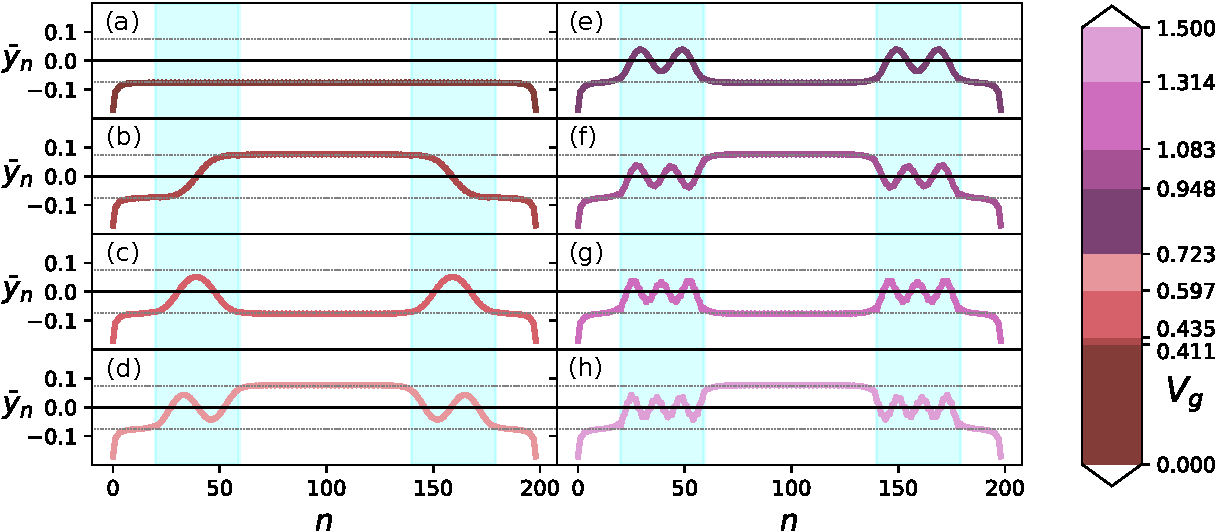
\includegraphics[scale=0.7]{figures/DWs.pdf}
    \caption{Staggered (lattice) distortion profiles $\bar{y}_{n}$ for the distinct lowest-energy configurations (i.e., global minima) that occur at applied voltages $V_{g}$ up to $1.5 \, \textbf{eV}$. The segments with a constant value of $\bar{y}_{n}$ correspond to one of the two possible Peierls dimerization patterns of tPA. The color-shaded regions indicate the location of the voltage gates, meaning that these sites can have ${\mu_{n} \ne 0}$. In the gate regions, the points where $\bar{y}_{n}$ crosses zero correspond to the center of DWs. Observe that the number of DWs per gate changes in an abrupt and discrete way only at critical values of $V_{g}$, whereas all solutions within each voltage range of stability (color-coded according to the color bar on the right) have their profiles visibly unaffected. }
    \label{fig:DWs}
\end{figure}

Our main finding is the occurrence of discrete ground-state transitions in tPA, as we continuously varied the external gate voltages (${V_{g} \in[0,1.5] \,\, \textbf{eV}}$), characterized by the voltage-induced accumulation of quantized charge in the gate regions. These quantized jumps are related to the appearance of DWs within the gate regions.

As is well known\cite{Heeger88_Solitons_in_conducting_polymers,Su79_Solitons_in_polyacetylene,Su80_Dynamics_of_solitons_in_PA}, the intra-gap electronic properties of tPA are intimately related to the Peierls distortion profile of the unperturbed ground-state. It is customary to define the \textit{staggered} distortion as follows:
%
\begin{align}\label{eq:staggered_field}
\bar{y}_{n} \equiv & \, (-1)^{n} \left[ u_{n+1} - u_{n} \right] \nonumber\\
= & \, (-1)^{n} \left[ R_{n+1} - R_{n} - a \right]\, ,
\end{align}
%
where its fast oscillations have been removed via the factor $(-1)^{n}$. As a result, $\bar{y}_{n}$ is a smooth field on the scale of the lattice parameter $a$, which allows to identify the regions with a specific alternation pattern, and therefore the presence of DWs in the system (i.e., where $\bar{y}_{n}$ crosses zero). Due to the symmetry of the SSH model,under the change $u_n \to -u_n$ with a simultaneous gauge transformation $c_{n,s} \to (-1)^n c_{n,s}$, the values $\pm u_{0}$ are degenerate. Consequently, a region with a constant staggered field of ${\bar{y}_{n} = \pm 2 u_{0}}$ corresponds to one of the two possible Peierls-dimerization patterns of tPA. Either of these two uniform solutions leads to a gap of ${\Delta_{0} = 4 \alpha \left| u_{0} \right|}$ between the filled valence band and the empty conduction band, at ${T = 0}$. For the present case, we have determined the Peierls gap at ${V_{g} = 0}$ to be ${\Delta_{0} = 0.628 \, \textbf{eV}}$; this value will be used as a reference throughout this work.

In the absence of external voltages, and using the aforementioned parameters, we recovered a uniform profile with ${|\bar{y}_{n}| = 0.0755 \, \textbf{\AA}}$. This single-pattern configuration is robust to small changes in the chemical potential of the molecule, as this remained to be the only solution in the range of very low voltages, up to ${\approx 0.4 \, \textbf{eV}}$ (see Fig.~\ref{fig:DWs}(a)). Note that, even for the unperturbed system, we observe small depressions near the edges; these distortions are introduced by the stretching term (proportional to $\Gamma$) and should be ignored as they are of no physical significance far away from the edges.

As the external voltage $V_{g}$ is increased beyond a critical value of ${V_{g}^{[1]} \approx 0.411 \, \textbf{eV}}$, the system undergoes an abrupt transition to a different distortion profile containing a single DW \textit{per gate} (see Fig.~\ref{fig:DWs}(b)). The emergence of a DW corresponds to a voltage-induced quantum phase transition\cite{sachdev1999quantum}, which arises from the crossing of energy levels as the external perturbation is continuously varied. The energy crossing occurs at critical values of $V_{g}$ where two solutions, differing in the number of DWs per gate, become  degenerate. The abrupt transitions are a consequence of the minimization process, which always selects the solution with the lowest energy for a given value of $V_{g}$. In line with this, the solutions with a number of DWs different from that of the ground state can be regarded as molecular excited states. It is important to remark that these  excited states are local minima (i.e., stable solutions with energies greater than the lowest possible) that can be accessed by choosing appropriate initial seeds for the ion positions in the minimization process.

It is worth mentioning that, in tPA, a single DW can be modeled in the continuum limit ${a \rightarrow 0, } \, { N_{s} \rightarrow \infty }$, by the means of the massive Dirac equation\cite{Jackiw76_Jackiw_Rebbi_soliton, Su79_Solitons_in_polyacetylene, Takayama80_Continuum_model_for_PA, Heeger88_Solitons_in_conducting_polymers}, in which the distortion profile ${\bar{y}_{n} \rightarrow \Delta(x)}$, with ${x = na}$, can be interpreted as an effective sign-changing ``mass’’ term. For an infinite system with a DW centered at $x=0$, this mass term adopts the simple functional form ${\Delta(x) = 2 u_{0} \tanh (x / \xi )}$, where ${\xi = \hbar v_{F} / \Delta_{0}}$ is the width of the DW (with $v_{F}$ being the Fermi velocity of the massless Dirac fermions\cite{Heeger88_Solitons_in_conducting_polymers}. For ${x \rightarrow \pm \infty}$, $\Delta(x)$ is a solution that interpolates between the constant values $\pm 2 u_{0}$ corresponding to single Peierls dimerization patterns. This model predicts topological intra-gap electronic states that are localized at the DW within a distance $\xi$ and emerge at the Fermi energy (i.e., at ${\epsilon = 0}$) in the electronic spectrum. These bound states are able to accommodate an extra charge and/or spin\cite{Asboth16_Short_course_on_TIs}, giving rise to the celebrated soliton excitations in tPA. The distortion profile of Fig.~\ref{fig:DWs}(b), which contains one DW per gate separated by a distance ${L_{s} \gg \xi}$, can be successfully reproduced with the ansatz:
%
\begin{eqnarray}
\Delta (x) \approx -2 u_{0} \tanh\left( \frac{x - x_{g^{+}}}{\xi} \right) . \tanh \left( \frac{x - x_{g^{-}}}{\xi} \right), 
\end{eqnarray}
%
where $x_{g^{+}}$ and $x_{g^{-}}$ refer to the center of the respective gates. In other words, perturbing the tPA molecule via an external voltage favors the accumulation of excess charge bound to the gate regions, via the generation of CDWs. For the case at hand (see Fig.~\ref{fig:DWs}(b)), a positive charge ${Q_{g}^{+} = +e}$ becomes localized at the DW on $g^{+}$ and, because of the anti-symmetry of the external potential profile, a compensating negative CDW also emerged at $g^{-}$ with charge ${Q_{g}^{-} = -e}$, maintaining the overall charge neutrality. Interestingly, although the charge estimated from the solution electron density was found to be localized at the lattice sites of the DWs, as in what we recognize as CWDs, it was not possible to identify individual one-electron (bound) intra-gap state responsible for the excess charge in the molecular solution provided by our tight-binding SSH model, demonstrating the collective nature of the charge localization phenomenon. % this fact can be deduced from Fig.~\ref{fig:eigenenergies}.

%
\begin{figure}
    \centering
    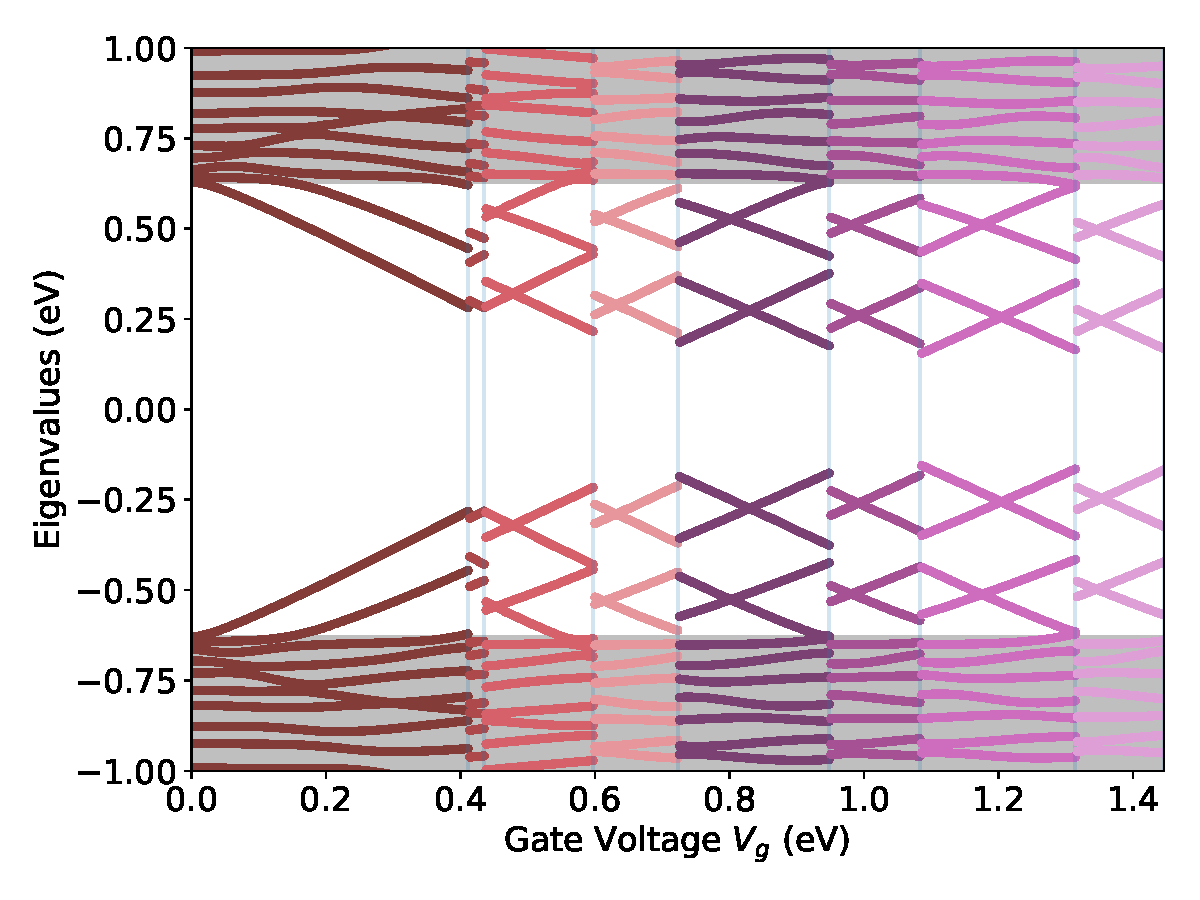
\includegraphics[scale=0.7]{figures/eigenenergies.pdf}
    \caption{ Single-particle energy spectrum (i.e. eigenvalues) of the lowest-energy solutions for applied voltages $V_{g}$ up to $1.5 \, \textbf{eV}$. Quantum phase transitions occur at critical values of $V_{g}$, which are also shown in the color bar of Fig.~\ref{fig:DWs}. The discontinuities in $V_{g}$ correspond to an abrupt change in the arrangement of the one-electron states, especially for those located within the Peierls gap (white background). Within each voltage range of stability (we use the same color coding as in Fig.~\ref{fig:DWs}), observe that the energy of the electronic states varies continuously with $V_{g}$; however, according to Fig.~\ref{fig:DWs}, these shifts in eigenvalues do not visibly affect the arrangement of the ions in the chain.}
    \label{fig:eigenenergies}
\end{figure}
%
Moreover, we find that this mechanism is not limited to the generation of a single excess charge per gate. We note that, by increasing the voltage even further, new critical values appear (${V_{g}^{[2]}, \, V_{g}^{[3]}, \, \dots}$), all corresponding to quantum transitions to solutions with an increasing integer number of CDWs per gate, i.e. with the respective number of localized, quantized excess charges per gate, as shown in Fig.~\ref{fig:DWs}(c-h).

To better visualize the abrupt nature of the quantum phase transitions, in Fig.~\ref{fig:eigenenergies} we show the evolution of the electronic spectrum around the energy gap, as a function of $V_{g}$. Here, the quantum phase transitions can be seen as abrupt changes in the electronic single-particle eigenenergies, with changes being more pronounced for the intra-gap states. Note that although the electronic spectrum varies even in regions of phase stability, the (lattice) distortion profile remains robust and visibly unaffected, meaning that its ability to accumulate charge via CDWs remains intact. Only a quantum transition, as the external potential is increased, can lead to a new configuration of ions capable of localizing more charge.
%
\begin{figure}
    \centering
    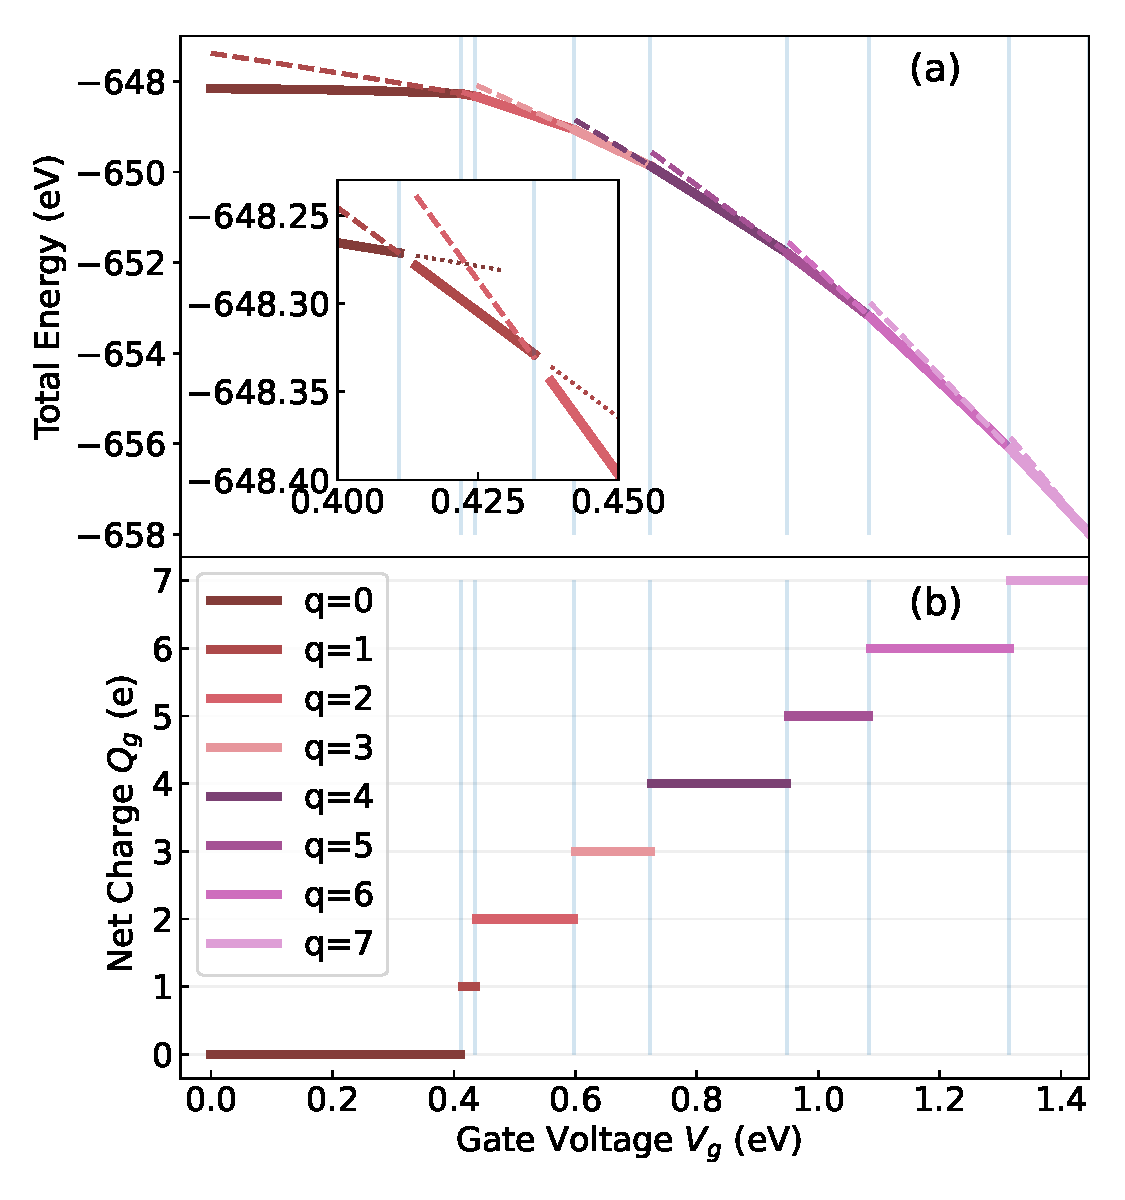
\includegraphics[scale=0.7]{figures/energy_and_charge.pdf}
    \caption{Total energy of the system (a) and absolute net charge per gate (b) as functions of applied voltage $V_{g}$. In both panels we use the same color coding as in Fig.~(\ref{fig:DWs}) to refer to the lattice configurations with a given number of DWs per gate. In panel (a), the solid lines correspond to the lowest-energy the system can be at each $V_{g}$. The dashed lines correspond to low-lying excited molecular states; since these are local minima, these states can be reached by starting from initial ion positions close to the desired non-optimal configuration. Notice how the quantum phase transitions occur at critical voltages, i.e. where there is a crossing of energy levels. In panel (b) we show the number of accumulated charges per gate from the CDWs present in the lowest-energy configuration for each $V_{g}$. To compute these values, we integrated the excess charge per site (see Section~A of the supplementary material) for a gate region and took its absolute value, resulting in an equal value of charge for both gates. In practice, a small number of sites immediately outside the gates had to be included in the integration in order to cancel out a very small charge contribution coming from spurious dipoles appearing at the sharp discontinuities in $V_{g}$. These artifacts have no physical significance for the modeled system and dissipate as the perturbation profile becomes smoother (not shown).
}
\label{fig:energy_and_charge}
\end{figure}
%
To emphasize the quantized nature of the accumulated charge, as an argument in favor of the topological origin of these transitions being the formation of voltage-induced CWDs, in Figs.~\ref{fig:energy_and_charge}(a) and (b) we show, respectively, as functions of the applied voltage $V_{g}$, the total energy of the system (i.e., electronic plus lattice) and the absolute net charge contained at each gate region. In panel (a) we can visualize the energy of the lowest configuration (thick lines) for each voltage stability range. In addition, note the occurrence of level crossings giving rise to quantum phase transitions, at (critical) voltage values, as we discussed above. In panel (b) we can see that the charge contained in each gate region is a strictly constant integer value between transition voltages. These quantized charges are associated with different solitonic phases of tPA and are as robust to changes in $V_{g}$ as the lattice profile of the  stable configuration, which is consistent with the gate net charge coming from the CWDs. There exists a simple analytical link between the two panels of Fig.~\ref{fig:energy_and_charge}, as the absolute excess charge per gate $Q_{g}$ can be obtained by deriving the total energy $E_{\textbf{GS}}$ with respect to the external potential $V_{g}$, making use of the Hellman Feynman theorem:
%
\begin{align}
\frac{\partial E_{\mathrm{GS}}}{\partial V_{g}} = & \left\langle \Psi_{\mathrm{GS}} \left| \frac{\partial \hat{H}_{\textbf{el}}}{\partial V_{g}} \right| \Psi_{\mathrm{GS}} \right\rangle \, , \nonumber\\
= & -2 \, Q_{g},\label{eq:localized_charge}
\end{align}
%
where the factor 2 is obtained due to the symmetry of the perturbation, as shown in Section~A of the supplementary material (SM). The remarkable simplicity of this expression is related to the fact that the capacitive coupling term contributes to the total energy as the electrostatic potential energy of the charges accumulated per gate due to the applied external voltage. 

In Section~B of the SM, we provide evidence that the perturbed molecular solutions are not only robust over a range of voltages (see e.g. Fig.~\ref{fig:energy_and_charge}(b)), but also to strong noise in the applied voltage profile $\mu_{n}$, which may originate from normal room temperature fluctuations or aspects related to the non-ideality of an experimental setup.

\section{Summary and Conclusions}\label{sec:conclusions}

From a theoretical perspective, we have discussed the design and feasibility of a proposed tPA-based nano-device capable of accumulating localized discrete charges in a controllable manner via external voltage gates. We attributed the quantized nature of the charges on each gate to the voltage-induced generation of CDWs, occurring thanks to the large intrinsic electron-phonon coupling of $\pi$-conjugated molecules. The appearance of CDWs is associated with quantum phase transitions due to energy level crossings between stable solutions with different numbers of DWs in their lattice staggered field profiles. We found that although these solutions are stable for a range of voltages and even to strong noise in the external perturbation, their electronic spectra are highly sensitive to changes in the external potential, providing a way to induce and control the energy of the topological intra-gap states. Overall, the proposed device is comparable to a semiconductor quantum dot (QD), but more robust and with highly localized charges. A significant difference with the so-called ``Coulomb diamonds'' in QD circuits is that the stability of the quantized charges does not come from Coulomb interactions, but from the robustness of the DWs.

Although building single-molecule electronic devices is certainly a real experimental challenge, we believe that the proposed device may be within reach in the near future, as there have been several recent advances in the on-surface synthesis of $\pi$-conjugated molecules\cite{Grill2007, Shen17_Frontiers_on_surface_review,Han21_Surface_assisted_fabrication_low_dimensional_carbon_nanostructures}, which can be observed and controlled with modern EBL-, AFM-, and STM-based techniques\cite{Wang19_Solitons_in_individual_PA_molecules}. Recent theoretical modeling also supports the possibility of designing single-molecule electronics\cite{Yao19_Unconventional_nanofabrication_supramolecular_electronics}, which could even be based on conductive polymers other than tPA\cite{cirera2020tailoring}.

While the anti-symmetry of the external voltage profile was just a trick to simplify our theoretical calculations, we emphasize that this is not a necessary condition for any experimental setup. In other words, our results can be easily extrapolated to the case of a single gate in open conditions, in which case the tPA molecule would have to be weakly coupled to an electron reservoir that allows $N_\text{el}$ to fluctuate (e.g., a metallic contact). Grand-canonical ensemble calculations would require the inclusion an explicit coupling to a reservoir; this is the subject of our subsequent line of research which is currently underway. Although our simple model neglects an explicit treatment of electron-electron interactions, given the remarkable energy difference between the ground- and low-lying excited-states, we do not expect our results (or conclusions) to change qualitatively, even in cases with strong correlations; this is also an argument for the stability of the configurations in a room-temperature scenario. In fact, rather than being a detrimental feature, the ability to induce strong correlations could open up new interesting possibilities for the device, involving exotic ground states, such as the generation of localized magnetic moments or the Kondo effect. For example, recent experiments have shown the presence of superconductivity in $\alpha$-terphenyl polymers upon doping \cite{Zhong18_Superconductivity_in_p_terphenyl, Yan19_Superconductivity_in_p_quaterphenyl, Huang19_Superconductivity_in_p_terphenyl}
, and strong correlations have been invoked to explain these interesting results.

In conclusion, and in light of our results, it becomes tempting to imagine the many exciting ways in which the presented mechanism for generating an arbitrary number of quantized excess charges at desired locations could be exploited in the design and development of next-generation tPA-based nano-devices.

\section*{Acknowledgements}
This work was supported by CONICET and Agencia
I + D + i under PICT 2017-2081, Argentina.

% References
\begin{thebibliography}{10}

\bibitem{Asboth16_Short_course_on_TIs}
J.K. Asb{\'o}th, L.~Oroszl{\'a}ny, and A.P. P{\'a}lyi.
\newblock {\em A Short Course on Topological Insulators: Band Structure and
  Edge States in One and Two Dimensions}.
\newblock Lecture Notes in Physics. Springer International Publishing, 2016.

\bibitem{Bernevig_book_TI_TSC}
B.~Andrei Bernevig and Taylor~L. Hughes.
\newblock {\em Topological Insulators and Topological Superconductors}.
\newblock Princeton University Press, 2013.

\bibitem{blanchet1983photoexcitations}
Graciela~B Blanchet, C.~R. Fincher, T.~C. Chung, and A.~J. Heeger.
\newblock Photoexcitations in trans-(ch) x: a fourier-transform infrared study.
\newblock {\em Physical review letters}, 50(24):1938, 1983.

\bibitem{Chiang77}
C.~K. Chiang, C.~R. Fincher, Y.~W. Park, A.~J. Heeger, H.~Shirakawa, E.~J.
  Louis, S.~C. Gau, and Alan~G. MacDiarmid.
\newblock Electrical conductivity in doped polyacetylene.
\newblock {\em Phys. Rev. Lett.}, 39:1098--1101, Oct 1977.

\bibitem{cirera2020tailoring}
Borja Cirera, Ana S{\'a}nchez-Grande, Bruno de~la Torre, Jos{\'e} Santos,
  Shayan Edalatmanesh, Eider Rodr{\'\i}guez-S{\'a}nchez, Koen Lauwaet, Benjamin
  Mallada, Radek Zbo{\v{r}}il, Rodolfo Miranda, et~al.
\newblock Tailoring topological order and $\pi$-conjugation to engineer
  quasi-metallic polymers.
\newblock {\em Nature Nanotechnology}, 15(6):437--443, 2020.

\bibitem{Farchioni_Grosso_Organic_electronic_metals_book}
R.~Farchioni, G.~Grosso, and (Eds).
\newblock {\em Organic Electronic Materials. Conjugated Polymers and Low
  Molecular Weight Organic Solids}.
\newblock Springer-Verlag, Berlin Heidelberg GmbH, Germany, 2001.

\bibitem{feynman39}
R.~P. Feynman.
\newblock {\em Phys. Rev.}, 56:340, 1939.

\bibitem{goldberg1979electron}
IB~Goldberg, HR~Crowe, PR~Newman, AJ~Heeger, and AG~MacDiarmid.
\newblock Electron spin resonance of polyacetylene and asf5-doped
  polyacetylene.
\newblock {\em The Journal of Chemical Physics}, 70(3):1132--1136, 1979.

\bibitem{Grill2007}
Leonhard Grill, Matthew Dyer, Leif Lafferentz, Mats Persson, Maike~V. Peters,
  and Stefan Hecht.
\newblock Nano-architectures by covalent assembly of molecular building blocks.
\newblock {\em Nature Nanotechnology}, 2(11):687--691, Nov 2007.

\bibitem{Han21_Surface_assisted_fabrication_low_dimensional_carbon_nanostructures}
Dong Han and Junfa Zhu.
\newblock Surface-assisted fabrication of low-dimensional carbon-based
  nanoarchitectures.
\newblock {\em Journal of Physics: Condensed Matter}, 33, 07 2021.

\bibitem{Heeger88_Solitons_in_conducting_polymers}
A.~J. Heeger, S.~Kivelson, J.~R. Schrieffer, and W.~P. Su.
\newblock Solitons in conducting polymers.
\newblock {\em Rev. Mod. Phys.}, 60:781--850, Jul 1988.

\bibitem{HernangomezPerez20_Solitonics_with_PA}
Daniel Hernangómez-Pérez, Suman Gunasekaran, Latha Venkataraman, and
  Ferdinand Evers.
\newblock Solitonics with polyacetylenes.
\newblock {\em Nano Letters}, 20(4):2615--2619, 2020.
\newblock PMID: 32125870.

\bibitem{Huang19_Superconductivity_in_p_terphenyl}
Ge~Huang, Guo-Hua Zhong, Ren-Shu Wang, Jia-Xing Han, Hai-Qing Lin, and Xiao-Jia
  Chen.
\newblock Superconductivity and phase stability of potassium-doped
  p-quinquephenyl.
\newblock {\em Carbon}, 143:837--843, 2019.

\bibitem{Jackiw76_Jackiw_Rebbi_soliton}
R.~Jackiw and C.~Rebbi.
\newblock Solitons with fermion number ½.
\newblock {\em Phys. Rev. D}, 13:3398--3409, Jun 1976.

\bibitem{Jiang18_Manipulation_of_DWs_in_bi_and_trilayer_graphene}
Lili Jiang, Sheng Wang, Zhiwen Shi, Chenhao Jin, M.~Iqbal~Bakti Utama, Sihan
  Zhao, Yuen-Ron Shen, Hong-Jun Gao, Guangyu Zhang, and Feng Wang.
\newblock Manipulation of domain-wall solitons in bi- and trilayer graphene.
\newblock {\em Nature Nanotechnology}, 13(3):204--208, Mar 2018.

\bibitem{park2022creation}
Jae~Whan Park, Euihwan Do, Jin~Sung Shin, Sun~Kyu Song, Oleksandr Stetsovych,
  Pavel Jelinek, and Han~Woong Yeom.
\newblock Creation and annihilation of mobile fractional solitons in atomic
  chains.
\newblock {\em Nature nanotechnology}, 17(3):244--249, 2022.

\bibitem{sachdev1999quantum}
Subir Sachdev.
\newblock Quantum phase transitions.
\newblock {\em Physics world}, 12(4):33, 1999.

\bibitem{sethna1982photoinduced}
James~P Sethna and Stephen Kivelson.
\newblock Photoinduced soliton pair production in polyacetylene: An instanton
  approach.
\newblock {\em Physical Review B}, 26(6):3513, 1982.

\bibitem{Shen17_Frontiers_on_surface_review}
Qian Shen, Hong-Ying Gao, and Harald Fuchs.
\newblock Frontiers of on-surface synthesis: From principles to applications.
\newblock {\em Nano Today}, 13:77--96, 2017.

\bibitem{Su80_Dynamics_of_solitons_in_PA}
W.~P. Su and J.~R. Schrieffer.
\newblock Soliton dynamics in polyacetylene.
\newblock {\em Proceedings of the National Academy of Sciences},
  77(10):5626--5629, 1980.

\bibitem{Su79_Solitons_in_polyacetylene}
W.~P. Su, J.~R. Schrieffer, and A.~J. Heeger.
\newblock {\em Phys. Rev. Lett.}, 42:1698--1701, Jun 1979.

\bibitem{Takayama80_Continuum_model_for_PA}
Hajime Takayama, Y.~R. Lin-Liu, and Kazumi Maki.
\newblock Continuum model for solitons in polyacetylene.
\newblock {\em Phys. Rev. B}, 21:2388--2393, Mar 1980.

\bibitem{Vanderbilt80_Disorder_in_tPA}
David Vanderbilt and Eugene~J. Mele.
\newblock Effects of disorder on the electronic structure of undoped
  polyacetylene.
\newblock {\em Phys. Rev. B}, 22:3939--3948, Oct 1980.

\bibitem{Vos96_SSH_model_finite_length}
Fernando L.~J. Vos, Daniel~P. Aalberts, and Wim~van Saarloos.
\newblock Su-schrieffer-heeger model applied to chains of finite length.
\newblock {\em Phys. Rev. B}, 53:14922--14928, Jun 1996.

\bibitem{Wang19_Solitons_in_individual_PA_molecules}
Shiyong Wang, Qiang Sun, Oliver Gr{\"o}ning, Roland Widmer, Carlo~A. Pignedoli,
  Liangliang Cai, Xin Yu, Bingkai Yuan, Can Li, Huanxin Ju, Junfa Zhu, Pascal
  Ruffieux, Roman Fasel, and Wei Xu.
\newblock On-surface synthesis and characterization of individual polyacetylene
  chains.
\newblock {\em Nature Chemistry}, 11(10):924--930, Oct 2019.

\bibitem{weinberger1980electron}
BR~Weinberger, E~Ehrenfreund, A~Pron, AJ~Heeger, and AG~MacDiarmid.
\newblock Electron spin resonance studies of magnetic soliton defects in
  polyacetylene.
\newblock {\em The Journal of Chemical Physics}, 72(9):4749--4755, 1980.

\bibitem{Yan19_Superconductivity_in_p_quaterphenyl}
Jia-Feng Yan, Guo-Hua Zhong, Ren-Shu Wang, Kai Zhang, Hai-Qing Lin, and
  Xiao-Jia Chen.
\newblock Superconductivity and phase stability of potassium-intercalated
  p-quaterphenyl.
\newblock {\em The Journal of Physical Chemistry Letters}, 10(1):40--47, 2019.

\bibitem{Yao19_Unconventional_nanofabrication_supramolecular_electronics}
Yifan Yao, Lei Zhang, Emanuele Orgiu, and Paolo Samorì.
\newblock Unconventional nanofabrication for supramolecular electronics.
\newblock {\em Advanced Materials}, 31(23):1900599, 2019.

\bibitem{Zhong18_Superconductivity_in_p_terphenyl}
Guo-Hua Zhong, Dong-Yu Yang, Kai Zhang, Ren-Shu Wang, Chao Zhang, Hai-Qing Lin,
  and Xiao-Jia Chen.
\newblock Superconductivity and phase stability of potassium-doped biphenyl.
\newblock {\em Phys. Chem. Chem. Phys.}, 20:25217--25223, 2018.

\end{thebibliography}

\end{document}